\chapter{Θεωρητικό υπόβαθρο}
\label{ch:theoreteical_background}

\section{Νευρωνικά δίκτυα}
Το νευρωνικό δίκτυο με την αφηρημένη έννοια του είναι μια δομή η οποία θα μπορούσε να χαρακτηριστεί ως ένας μηχανισμός αριθμητικών πράξεων με συνήθως περισσότερες από μια εισόδους και μια ή περισσότερες εξόδους. Ένα νευρωνικό δίκτυο αποτελείται από τους κόμβους--νευρώνες του (\tl{\textbf{nodes}}) οι οποίοι ενώνονται μέσω των συνάψεων του. Το σύνολο των κόμβων οι οποίοι συνδέονται με τις ίδιες ομάδες συνάψεων λέγεται επίπεδο (\tl{\textbf{layer}}).

Η στατική μορφή ενός νευρωνικού δικτύου ως μηχανισμό εξαγωγής αποτελεσμάτων αριθμητικών πράξεων ή αλλιώς η πρόβλεψη ενός μοντέλου αποτελεί μια απλή διαδικασία όπου το αποτέλεσμα κάθε κόμβου πολλαπλασιάζεται με τα βάρη των συνάψεων και εισέρχεται στους κόμβους του επόμενου επιπέδου σαν είσοδος. Ο συγκεκριμένος μηχανισμός ενός νευρωνικού δικτύου ονομάζεται διάδοση προς τα εμπρός (\tl{\textbf{forward propagation}}).

Ένας ακόμη σημαντικός μηχανισμός που κάνει ένα νευρωνικό δίκτυο ένα χρήσιμο εργαλείο είναι αυτός που δίνει τη δυνατότητα τροποποίησης των βαρών του με αποτέλεσμα την εκπαίδευση του μοντέλου. Ο τρόπος με τον οποίο το παραπάνω είναι εφικτό είναι με μια αντίστροφη διαδικασία από την διάδοση προς τα εμπρός, δηλαδή με βάση μια επιθυμητή τιμή εξόδου τα βάρη του μοντέλου προσαρμόζονται από τα τελευταία προς τα πρώτα επίπεδα, με σκοπό να μειωθεί το σφάλμα ως προς την επιθυμητή έξοδο. Η διαδικασία αυτή ονομάζεται οπισθοδιάδοση \tl{(\textbf{backpropagation})}.

\begin{figure}[H]
  \begin{center}
    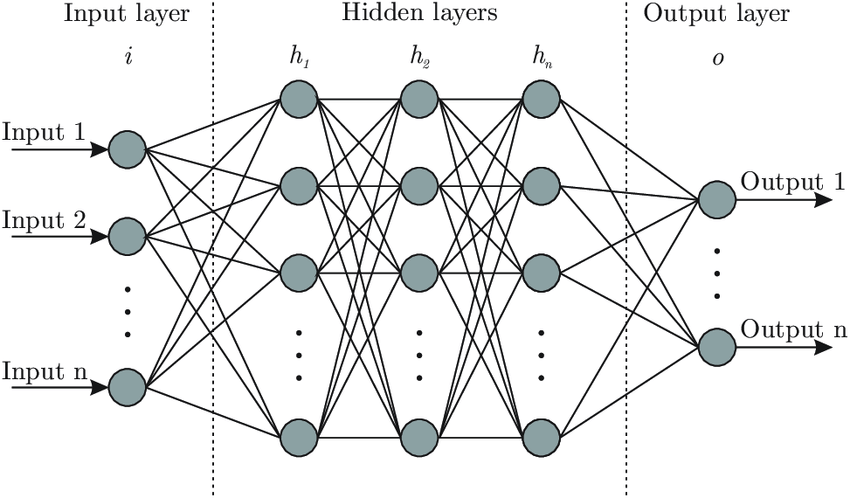
\includegraphics[width=0.8\textwidth]{THEORETICAL_BACKGROUND/neural_network.png}
    \caption{Γενική μορφή Νευρωνικού δικτύου (Πηγή: \href{https://mc.ai/my-notes-on-neural-networks-2/}{\tl{mc.ai}})}
    \label{fig:neur_net}
  \end{center}
\end{figure}

Για τη σωστή λειτουργία ενός νευρωνικού δικτύου είναι απαραίτητοι ορισμένοι επιπλέον μηχανισμοί οι οποίοι μετασχηματίζουν τις τιμές εξόδου των κόμβων --- αυτές είναι οι συναρτήσεις ενεργοποίησης. Μια από τις συναρτήσεις ενεργοποίησης οι οποίες χρησιμοποιούνται συνήθως είναι η ανορθωμένη γραμμική συνάρτηση. \todo{κάποιες (πληθυντικός) έχεις μόνο τη ReLU. Επίσης όχι έξτρα υποενότητα (3.1.1) αν δεν υπάρχει 3.1.2}

\subsection{Ανορθωμένη γραμμική συνάρτηση \tl{(ReLU)}}
Η ανορθωμένη γραμμική συνάρτηση \tl{ReLU (Rectified Linear Unit)} είναι ουσιαστικά η γραμμική συνάρτηση $\mathit{\mathbf{f\left(x\right) = x}}$, η οποία είναι τροποποιημένη στο μέρος της αρνητικής εισόδου της ώστε να μηδενίζει την έξοδο. Η χρήση της είναι συνήθης στην δομή των νευρωνικών δικτύων ως συνάρτηση ενεργοποίησης, λόγω της ιδιότητας της να αποκόπτει αρνητικές τιμές κατά την διάδοση των σημάτων μεταξύ των κόμβων--νευρώνων, κάτι που επιτρέπει την ομαλή εκπαίδευση του.

\begin{figure}[H]
  \begin{center}
    \includesvg[width=1\textwidth]{THEORETICAL_BACKGROUND/ReLU}
    \caption{Μορφή της συνάρτησης ανορθωμένης γραμμικής συνάρτησης \tl{ReLU}}
  \end{center}
\end{figure}

\section{Συνελικτικά Νευρωνικά Δίκτυα}
Τα Συνελικτικά Νευρωνικά Δίκτυα αποτελούν μια συγκεκριμένη μορφή των νευρωνικών δικτύων τα οποία περιλαμβάνουν επίπεδα στα οποία οι κόμβοι δεν είναι πλήρως συνδεδεμένοι με κάθε κόμβο του επομένου επιπέδου αλλά είναι μόνο με ορισμένους που ανήκουν σε μια περιοχή. 

Επίσης χρησιμοποιούνται ορισμένοι ακόμη τύποι επιπέδων όπως για παράδειγμα την τροποποίηση των διαστάσεων της εισόδου με συγκέντρωση μεγίστων (\tl{\textbf{Max Pooling}}).

Στις επόμενες υποενότητες θα αναλυθούν τα επιμέρους τμήματα που χρησιμοποιούνται σε ένα συνελικτικό νευρωνικό δίκτυο.

\section{Διαδικασία εκπαίδευσης συνελικτικού νευρωνικού δικτύου}\todo{Μήπως κάτω από το κεφάλαιο του \tl{CNN};}
Κατά την εκπαίδευση ενός συνελικτικού νευρωνικού δικτύου γίνεται χρήση του αλγορίθμου οπισθοδιάδοσης, έτσι το σφάλμα που παρατηρείται στην έξοδο χρησιμοποιείται για την ρύθμιση των βαρών των πλήρως συνδεδεμένων επιπέδων, ενώ στη συνέχεια καθώς η διόρθωση των βαρών των επιπέδων κινείται προς τα πρώτα επίπεδα, ρυθμίζον ται οι τιμές των παραμέτρων των συνελικτικών φίλτρων των αντίστοιχων επιπέδων για όλο το σύνολο των φίλτρων που περιλαμβάνουν.\\

Ο ρυθμός τροποποίησης των βαρών κάθε επιπέδου είναι επιθυμητό να γίνεται με έναν τρόπο κατά τον οποίο το συνελικτικό νευρωνικό δίκτυο θα εκπαιδεύεται με ικανοποιητικό ρυθμό, ώστε να μην υπάρχει υποεκπαίδευση. Ωστόσο επιπλέον η μεταβολή των βαρών δεν πρέπει να γίνεται πολύ γρήγορα ειδάλλως υπάρχει ταλάντωση στο σφάλμα εκπαίδευσης και είναι πιθανό να μην μπορεί να συγκλίνει σε κάποιο ελάχιστο σημείο. Με βάση τα παραπάνω φαίνεται πως απαιτείται ένας μηχανισμός ο οποίος θα επιβλέπει τον ρυθμό μεταβολής των βαρών τόσο κατά την εκκίνηση της εκπαίδευσης όσο και στην εξέλιξη της.

\subsection{Δισδιάστατα Συνελικτικά Επίπεδα}
Τα δισδιάστατα συνελικτικά νευρωνικά δίκτυα είναι γνωστά για τις εφαρμογές τους οι οποίες είναι σχετικές με την εικόνα. Μια συνήθης χρήση των συνελικτικών νευρωνικών δικτύων είναι η ταξινόμηση εικόνων με βάση το αν περιλαμβάνουν ένα συγκεκριμένο αντικείμενο. Μια ακόμη χρήση είναι η αναγνώριση προσώπου, δηλαδή η εξαγωγή χαρακτηριστικών του προσώπου με σκοπό την ταυτοποίηση ενός ατόμου. Παρόμοια είναι επίσης η εφαρμογή της αναγνώρισης των χαρακτηριστικών γραφής. \todo{Μπορείς να βάλεις καμία παράγραφο που έχουν εφαρμοστεί (π.χ. ταξινόμηση εικόνων). Είναι δύο διαστάσεων η είσοδος, το φάσμα είναι μία. Κάνε μία νύξη για αυτό}
Η είσοδος που χρησιμοποιείται στο μοντέλο πρόβλεψης αυτής της διπλωματικής εργασίας είναι ένα σπεκτρόγραμμα το οποίο είναι είσοδος 2 διαστάσεων, σε αντίθεση με άλλες υλοποιήσεις στις οποίες χρησιμοποιείται συνελικτικό νευρωνικό δίκτυο με είσοδο το φάσμα το οποίο είναι ένα μονοδιάστατο σήμα.\\

Τα συνελικτικά επίπεδα είναι το χαρακτηριστικό μέρος των συνελικτικών δικτύων, όπως προδίδει το όνομα τους αποτελούν τμήματα τα οποία μετασχηματίζουν και εξάγουν από την είσοδο πληροφορία με βάση την εφαρμογή συνελικτικών φίλτρων. Η διαδικασία αυτή επιτρέπει την εξαγωγή χρήσιμης πληροφορίας προς τα επόμενα επίπεδα για την ανίχνευση πιθανών μοτίβων ενώ ταυτόχρονα δεν απαιτεί το μέγεθος των πυκνών \tl{dense} επιπέδων καθώς αφορά πράξεις ενός σημείου της εισόδου με ορισμένα γειτονικά σημεία και όχι την μέθοδο πράξεων σημεία όλα προς όλα.

Η μορφή της περιοχής των γειτονικών σημείων καθορίζεται από το φίλτρο \tl{\textbf{Kernel}} που χρησιμοποιείται. Ο πυρήνας που χρησιμοποιείται συνήθως σε δισδιάστατα νευρωνικά δίκτυα είναι διαστάσεων $3\times3$. Ορισμένες ακόμη παράμετροι των πυρήνων είναι ο αριθμός των φίλτρων που υπάρχουν στο συγκεκριμένο επίπεδο αλλά και ο τρόπος που εφαρμόζονται τα συνελικτικά φίλτρα. Η πρώτη παράμετρος είναι το βήμα συνέλιξης ως προς τις 2 διαστάσεις, το οποίο συνήθως είναι μονάδα, ενώ για τιμές μεγαλύτερες της μονάδας υπάρχει υποδειγματοληψία για το επόμενο επίπεδο. Επίσης κατά την εφαρμογή συνελικτικών φίλτρων υπάρχει η επιλογή συνέλιξης στα άκρα του δισδιάστατου επιπέδου ώστε το συνελικτικό φίλτρο να χωράει πάντα μέσα στην εικόνα, ή η επιλογή συνέλιξης και σε ορισμένα σημεία εκτός της εικόνας με την προσθήκη μηδενκών ώστε το αποτέλεσμα της συνέλιξης να έχει ίδιες διαστάσεις με την αρχική εικόνα.

Κατά την εφαρμογή ενός συνελικτικού επιπέδου στην είσοδο ή οποιοδήποτε ενδιάμεσο επίπεδο, κάθε συνελικτικό φίλτρο εφαρμόζεται σε όλη την έκταση της εικόνας σύμφωνα με τις παραμέτρους βήματος και την επιλογή για τα ακραία σημεία της εικόνας. Το αποτέλεσμα είναι μια εικόνα ίσων ή μικρότερων διαστάσεων και αριθμού καναλιών $\mathbf{N\times M}$ όπου $\mathbf{N}$ ο αριθμός των καναλιών της εικόνας εισόδου και $\mathbf{M}$ ο αριθμός των φίλτρων του συνελικτικού επιπέδου. Ο αριθμός των παραμέτρων εκπαίδευσης του συνελικτικού επιπέδου είναι ίσος με $\mathbf{\left(A \times B\times N+1\right)\times M}$ όπου $\mathbf{A}$ και $\mathbf{B}$ το πλάτος και ύψος του κάθε συνελικτικού φίλτρου.\\

Στην υλοποίηση που εξετάζεται χρησιμοποιούνται συνελικτικά επίπεδα 2 διαστάσεων καθώς η είσοδος του δικτύου όπως θα αναφερθεί προκύπτει ως εικόνα ενός καναλιού έπειτα από μετασχηματισμό του αρχικού σήματος.

\subsection{Πλήρως συνδεδεμένα επίπεδα}
Η χρήση των πλήρως συνδεδεμένων επιπέδων είναι απαραίτητη για την αποτελεσματική πρόβλεψη ενός συνελικτικού νευρωνικού δικτύου. Η τοποθέτηση τους στην δομή του μοντέλου ωστόσο προτιμάται να γίνεται σε σημεία όπου η διαστάσεις του προηγούμενου επιπέδου είναι σχετικά μικρές και η επεξεργασία του συγκεκριμένου επιπέδου αφορά την εκτίμηση της προηγουμένως επεξεργασμένης εισόδου. Η μορφή ενός πλήρως συνδεδεμένου επιπέδου είναι αυτή των κρυφών (\textbf{\tl{Hidden}}) επιπέδων του σχήματος \ref{fig:neur_net}.

Στην αρχιτεκτονική των νευρωνικών δικτύων που πραγματεύεται η παρούσα εργασία τα πλήρως συνδεδεμένα επίπεδα τοποθετούνται μετά από τα συνελικτικά επίπεδα και ακριβώς πριν την έξοδο.

\subsection{Επίπεδα κανονικοποίησης παρτίδας(\tl{Batch Normalization})}
Η χρησιμότητα των επιπέδων κανονικοποίησης παρτίδας είναι στην εκπαίδευση των νευρωνικών και έχει ως σκοπό την αποφυγή της συνδιακυμαίνουσας μετατόπισης. Η συνδιακυμαίνουσα μετατόπιση είναι ένα φαίνόμενο που οφείλεται στις τροποποιήσεις των παραμέτρων των συνελικτικών επιπέδων με αποτέλεσμα την διακύμανση των εξόδων τους.\\

Κατά την κανονικοποίηση παρτίδας τα δεδομένα τα οποία χρησιμοποιούνται κατά την εκπαίδευση μέσα σε μια εποχή χωρίζονται σε ομάδες ορισμένου μεγέθους το οποίο ονομάζεται μέγεθος παρτίδας (\tl{Batch Size}). Για κάθε παρτίδα τα δεδομένα κανονικοπούνται πριν από τις συναρτήσεις ενεργοποίησης των συνελικτικών και πλήρως συνδεδεμένων επιπέδων ώστε να έχουν μέση τιμή μηδέν και διακύμανση μονάδα.

Ένα βασικό όφελος που προκύπτει από την χρήση της κανονικοποίηση παρτίδας, είναι η επιτάχυνση της διαδικασίας της εκπαίδευσης μέσω της παράλληλης επεξεργασίας των δειγμάτων με την χρήση της κάρτας γραφικών ενός υπολογιστικού συστήματος.

\subsection{Επίπεδα \tl{Dropout}}
Η μέθοδος \tl{Dropout} αποσκοπεί σε μια πιο εύρωστη εκπαίδευση ενός νευρωνικού δικτύου. Ο τρόπος με τον οποίο λειτουργεί είναι με την τυχαία απενεργοποίηση νευρώνων με αποτέλεσμα την αναγκαστική εκπαίδευση εναλλακτικών νευρώνων, δηλαδή αποφεύγεται η υπερενεργοποίηση συγκεκριμένων νευρώνων για συγκεκριμένες εισόδους όπως επίσης και η αδρανοποίηση ορισμένων νευρώνων οι οποίοι ενδεχομένως να ήταν πιο "τεμπέλικοι" εάν δεν χρησιμοποιούνταν η συγκεκριμένη τεχνική.

\subsection{Επίπεδα υποδειγματοληψίας --- Συγκέντρωση μεγίστων \tl{(Max Pooling)}}
Τα επίπεδα υποδειγματοληψίας είναι σημαντικά για τη δομή ενός συνελικτικού νευρωνικού δικτύου καθώς μειώνουν τις διαστάσεις την διάσταση της εισόδου μειώνοντας έτσι τον αριθμό των παραμέτρων του νευρωνικού δικτύου. Ταυτόχρονα η πληροφορία από τα σημεία της εισόδου που έχουν ενεργοποιηθεί δεν χάνεται. 

Κατά την εφαρμογή ενός επιπέδου συγκέντρωσης ορίζεται μια περιοχή συγκέντρωσης από τις τιμές της εισόδου σε αυτή την περιοχή θα εξαχθεί μια τιμή ανάλογα με τον τύπο επιπέδου συγκέντρωσης. Η διάσταση της περιοχής συγκέντρωσης είναι συνήθως $2\times2$. 

\begin{figure}[H]
  \begin{center}
    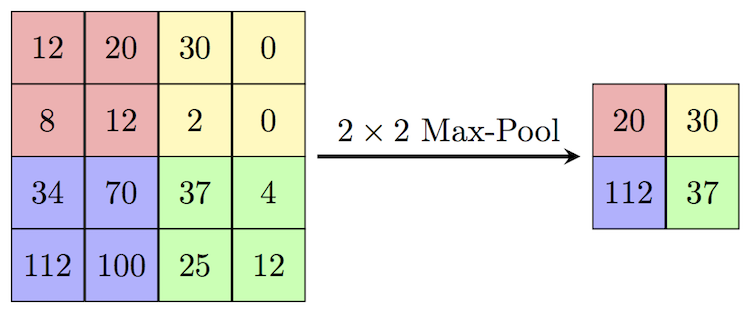
\includegraphics[width=0.7\textwidth]{THEORETICAL_BACKGROUND/max_pooling.png}
    \caption{Μέθοδος συγκέντρωσης μεγίστων για περιοχές διαστάσεων $2\times2$ (Πηγή: \href{https://computersciencewiki.org/index.php/Max-pooling_/_Pooling}{\tl{Computer Science Wiki}})}
  \end{center}
\end{figure}

Οι 2 τύποι επιπέδων υποδειγματοληψίας είναι τα συγκέντρωσης μεγίστων και συγκέντρωσης μέσης τιμής. Στην υλοποίηση που χρησιμοποιήθηκε παρατηρήθηκε πως η χρήση συγκέντρωσης μεγίστων έχει σημαντικά καλύτερη επίδοση σε σχέση με την συγκέντρωση μέσου όρου.

\subsection{Αρχικοποίηση Νευρωνικών Δικτύων}
Κατά την αρχικοποίηση ενός νευρωνικού δικτύου, η εκχώρηση των κατάλληλων βαρών των τεχνητών νευρώνων κάθε κόμβου παίζει σημαντικό ρόλο στην μετέπειτα δυνατότητα του μοντέλου να έχει μια στατιστικά αμερόληπτη κατάσταση εκκίνησης της εκπαίδευσης του, έτσι είναι εφικτό να τροποποιούνται τα βάρη του με κατάλληλο τρόπο ώστε να βελτιώνεται η απόδοση του κατά την διαδικασία της εκπαίδευσης.
Για τον παραπάνω σκοπό υπάρχουν ορισμένες μέθοδοι αρχικοποίησης των βαρών ενός μοντέλου
Ένας από του αρχικοποιητές που χρησιμοποιήθηκε για τα συνελικτικά φίλτρα είναι ο \tl{kernel\_initializer *random\_uniform*}. Οι αρχικές τιμές με τη χρήση του παραπάνω προκύπτουν από μια ομοιόμορφη κατανομή ενός ορισμένου εύρους τιμών. Η αρχικοποίηση των διανυσμάτων πόλωσης έγινε με τη χρήση του αρχικοποιητή
 \tl{bias\_initializer: zeros}, όπου οι αρχικές τιμές του διανύσματος πόλωσης ορίζονται μηδέν.

\subsection{Μέθοδοί ελαχιστοποίησης σφάλματος --- Βελτιστοποιητές \tl{(Optimizers)}}
Όπως προαναφέρθηκε η χρήση ενός μηχανισμού τροποποίησης του ρυθμού εκμάθησης και επίβλεψης του σφάλματος εκπαίδευσης είναι απαραίτητος για την επιτυχή εκπαίδευση ενός μοντέλου. 
\subsubsection{Στοχαστική κατάβαση δυναμικού \tl{SGD (Stochastic Gradient Descent)}}
Η πιο γνωστή μέθοδος ελαχιστοποίησης σφάλματος είναι η στοχαστική κατάβαση δυναμικού \tl{\textbf{SGD (Stochastic Gradient Descent)}}, η οποία αποτελεί μια απλή μέθοδο για την ελαχιστοποίηση του σφάλματος με βάση μια συνάρτηση σφάλματος η οποία στην περίπτωση των νευρωνικών δικτύων είναι συνήθως ένα άθροισμα των εισόδων ενός επιπέδου πολλαπλασιασμένων με τα βάρη τους. Η τρόπος με τον οποίο πραγματοποιείται η ελαχιστοποίηση της συνάρτησης είναι με τη χρήση της μερικής παραγώγου της ή αλλιώς την κλίση της. Για την μείωση της πολυπλοκότητας του αλγορίθμου η διαδικασία εκτελείται με στοχαστικό τρόπο, δηλαδή οι υπολογισμοί των παραγώγων δεν γίνονται για όλα τα σημεία του σετ δεδομένων αλλά επιλέγονται ορισμένα από αυτά με έναν τυχαίο τρόπο.
\subsubsection{Αλγόριθμος \tl{RMSprop}}
Ο \tl{RMSprop} είναι επίσης ένας γνωστός αλγόριθμος για την χρήση του σε βαθειά μηχανική μάθηση. Έχει ως βάση τον απλοποιημένο αλγόριθμο rprop όπου γίνεται χρήση της κλίσης αλλά και διαίρεση με αυτή έτσι εστιάζει κυρίως στη χρήση του προσήμου αυτής. Ωστόσο επειδή ο \tl{RMSprop} εφαρμόζεται σε μικρές ομάδες δειγμάτων, η υλοποίηση τροποποιείται με τη χρήση ενός κινητού μέσου όρου του τετραγώνου των κλίσεων κάθε βάρους ώστε να μπορεί να χρησιμοποιήθει σε όλα τα δείγματα. Το όνομα του αλγορίθμου προκύπτει από το χαρακτηριστικό του να διαιρεϊται η κλίση με την τετραγωνική ρίζα των μέσων τετραγώνων \tl{RMS}.
\subsubsection{Βελτιστοποιητής \tl{Adam}}
Μια από τις μεθόδους ελαχιστοποίησης σφάλματος η οποία παρατηρήθηκε πως είναι κατάλληλη για την χρήση σε συνελικτικά νευρωνικά δίκτυα είναι ο βελτιστοποιητής \tl{Adam (Adaptive Moment Estimation)}. Θα μπορούσε να θεωρηθεί ως ένας συνδυασμός των \tl{RMSprop} και \tl{SGD}. Ο τρόπος με τον οποίο μοιάζει με αυτούς τους 2 βελτιστοποιητές είναι ότι γίνεται χρήση των τετραγώνων της κλίσης για την κλιμακοποίηση του ρυθμού εκμάθησης όπως στον αλγόριθμο \tl{RMSprop}, ενώ επίσης χρησιμοποιεί το στοιχείο της ορμής με τη εφαρμογή ενός κινούμενου μέσου όρου της κλίσης, κάτι που μοιάζει με τον αλγόριθμο \tl{SGD} με ορμή.\\

Ο υπολογισμός της παραμέτρου 1ης και της 2ης ορμής αντίστοιχα γίνεται με βάση τους παρακάτω τύπους:
$$m_t=\beta_1m_{t-1}+\left(1-\beta_1\right)g_t$$
$$v_t=\beta_2v_{t-1}+\left(1-\beta_2\right)g_t^2$$

\subsubsection{Βελτιστοποιητής \tl{Nadam}}
Ένας ακόμη βελτιστοποιητής που χρησιμοποιείται είναι ο \tl{Nadam} ο οποίος πρόκειται για μια τροποποίηση του \tl{Adam} που συνδυάζει τον αλγορίθμου \tl{NAG (Nesterov accelerated SGD)}. Το χαρακτηριστικό του αλγορίθμου \tl{NAG} είναι πως δεν χρησιμοποιεί το τρέχον βήμα αλλά και το επόμενο, έτσι υπάρχει αξιοσημείωτη ελάττωση των ταλαντώσεων της καμπύλης του σφάλματος με επακόλουθο μια αποτελεσματικότερη εκπαϊδευση.\\

\section{Μέθοδος εξαγωγής \tl{Spectrogram}}
Το σπεκτρόγραμμα είναι μια δισδιάστατη αναπαράσταση ενός μονοδιάστατου σήματος όπου στον κατακόρυφο άξονα αποτυπώνεται το φασματικό περιεχόμενο μιας περιοχής του αρχικού σήματος. Η εξαγωγή των σπεκτρογραμμάτων συνήθως χρησιμοποιείται σε σήματα τα οποία είναι συνάρτηση του χρόνου με σκοπό την εξαγωγή χαρακτηρηστικών σχετικά με το φάσμα και την συχνότητα.\\
Για την εξαγωγή ενός σπεκτρογράμματος το αρχικό σήμα χωρίζεται σε ένα πλήθος $K$ τμημάτων με τη χρήση παραθύρων σταθερού μήκους $M$ δειγμάτων, χρησιμοποιώντας επικάλυψη $N$ ανάμεσα σε διαδοχικά παράθυρα. Σε κάθε τμήμα του γίνεται μετασχηματισμός Fourier μικρής χρονικής διάρκειας \tl{STFT (Short Time Fourier Transform)}. Έτσι το τελικό πλήθος των υποτμημάτων $K$, το οποίο θα είναι και η οριζόντια διάσταση του σπεκτρογράμματος, ορίζεται από την μορφή των παραθύρων αλλά και την επικάλυψη τους.\\
Οι διαστάσεις της μονοκαναλικής εικόνας που προκύπτουν είναι 
$$K=\lfloor\frac{X}{M-K}\rfloor+1$$
Σχήμα επικαλυπτώμενων παραθύρων σε ένα σήμα\\

Σχήμα αρχικής μορφής μονοδιάστατου σήματος---σπεκτρογράμματος του\\

Ο τύπος του παραθύρου που επιλέγεται ορίζει κατά κάποιον τρόπο τον αποτέλεσμα του μετασχηματισμού \tl{STFT}. Τα χαρακτηριστικά που έχει ένα παράθυρο που χρησιμοποιείται για την εξαγωγή σπεκτρογραμμάτων είναι η συμμετρία του ως προς το μέσον του, η ομαλή μετάβαση προς το μηδέν στα άκρα του και μια απόκριση στο φάσμα στην οποία να υπάρχουν κυρίως οι χαμηλότερες συχνότητες ενώ οι υψηλότερες να έχουν σημαντικά μικρότερη τιμή.

\begin{figure}[H]
  \begin{center}\selectlanguage{english}
    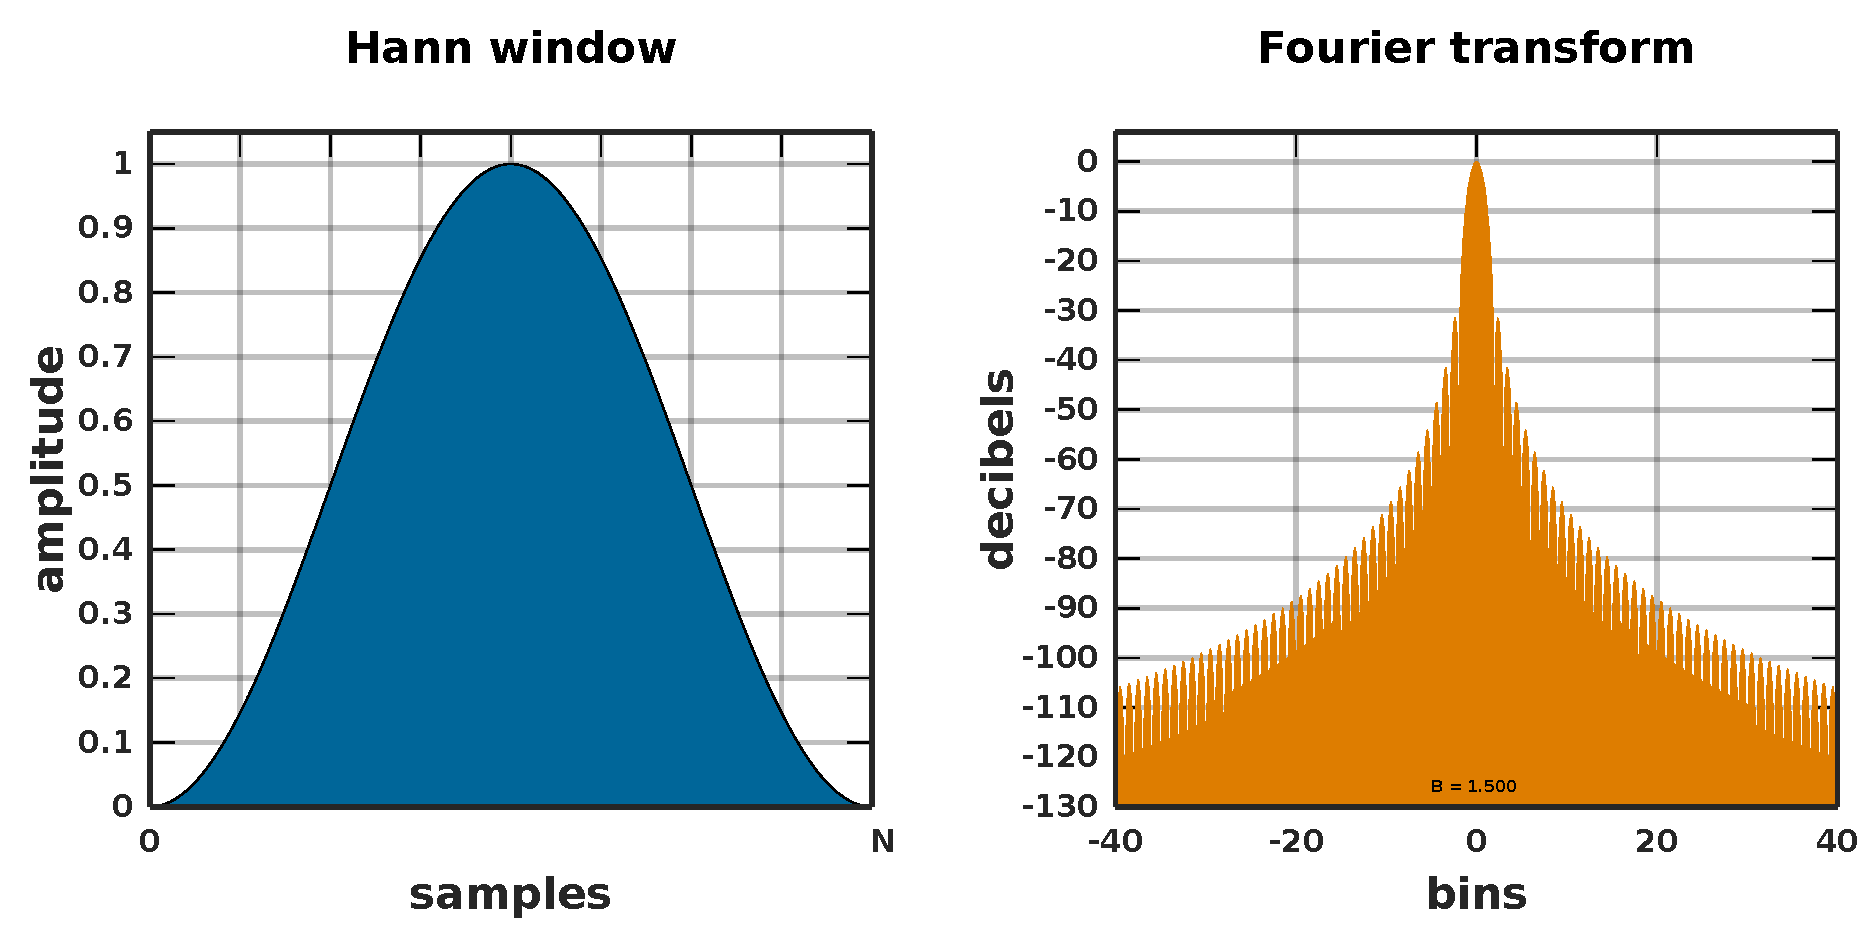
\includegraphics[width=1\textwidth]{THEORETICAL_BACKGROUND/HannWindow.pdf}
    \selectlanguage{greek}
    \caption{Απόκριση του παραθύρου \tl{Hann} στο χρόνο (αριστερά) και στη συχνότητα (δεξιά)}
  \end{center}
\end{figure}

\section{Μετασχηματισμός των \tl{Savitzky--Golay}}
Ο μετασχηματισμός των \tl{Savitzky--Golay}\cite{savitzky_golay} είναι μια μέθοδος εξομάλυνσης ενός σήματος. Ο τρόπος που εξάγεται είναι ουσιαστικά με τη χρήση μιας συνέλιξης κατά την οποία για κάθε δείγμα με τη χρήση των γειτονικών δειγμάτων του γίνεται εκτίμηση μιας καμπύλης του σήματος με τη χρήση πολυωνύμων μικρού βαθμού. Επίσης είναι μια συχνή στρατηγική ο μετασχηματισμός των tl{Savitzky--Golay} να χρησιμοποιείται για την εξαγωγή μιας εξομαλυσμένης μορφής της 1ης ή της 2ης παραγώγου ενός σήματος.\\

Σχήμα αρχικού---μετασχηματισμένου σήματος

\section{Μετρικές απόδοσης των μοντέλων}
Οι μετρικές αξιολόγησης που χρησιμοποιήθηκαν είναι το μέσο τετραγωνικό σφάλμα, η ρίζα του μέσου τετραγωνικού σφάλματος, ο συντελεστής προσδιορισμού και το ενδοτεραρτημοριακό εύρος. Είναι επιθυμητό κάθε μοντέλο να αξιολογείται με τη χρήση διαφορετικών μετρικών καθώς κάθε μια από αυτές εκφράζουν με ξεχωριστό τρόπο την επίδοση ενός μοντέλου και η χρησιμότητα τους μπορεί να διαφέρει ανάλογα με τις ιδιαιτερότητες της εξόδου που προβλέπεται.

\subsection{Μέσο τετραγωνκό σφάλμα}
Η μετρική του μέσου τετραγωνικού σφάλματος είναι μια από τις πιο συνήθεις για την εκπαίδευση και αξιολόγηση μοντέλων. Η χρησιμότητα της οφείλεται στο γεγονός πως η τετραγωνισμένες τιμές των σφαλμάτων τονίζουν περισσότερο τα μεγαλύτερα σφάλματα πρόβλεψης κάτι το οποίο είναι χρήσιμο κατά την εκπαίδευση. Ο τύπος υπολογισμού είναι ο παρακάτω.

$$MSE=\frac{1}{n}\sum_{i=1}^{n} {\left(x_{i}-\hat{x_{i}}\right)}^2$$

\subsection{Ρίζα του μέσου τετραγωνκού σφάλματος}
Η συγκεκριμένη μετρική είναι σχεδόν ίδια με το μέσο τετραγωνικό σφάλμα με την διαφορά ότι η τιμή της είναι πιο αντιπροσωπευτική ως προς το μέγεθος των τιμών της σε σχέση με τις τιμές της εξόδου.

$$RMSE=\sqrt{\frac{1}{n}\sum_{i=1}^{n} {\left(x_{i}-\hat{x_{i}}\right)}^2}$$
Όπου $\hat{x_{i}}$ είναι η πρόβλεψη του μοντέλου για την έξοδο $x_i$.

\subsection{Συντελεστής προσδιορισμού}
Ο συντελεστής προσδιορισμού \tl{Coefficient of Determination} είναι μια σημαντική μετρική με βάση την οποία προκύπτουν αρκετά από τα συμπεράσματα σχετικά με τις προβλέψεις των διαφόρων μοντέλων. Αυτό οφείλεται στο προκαθορισμένο εύρος τιμών της 0 εως 1 ανεξάρτητα από την έξοδο η οποία εξετάζεται και το σημαντικότερο πως δείχνει την ικανότητα ενός μοντέλου να κάνει ουσιαστικές προβλέψεις οι οποίες απέχουν από το μοντέλο που προβλέπει πάντα την μέση τιμή της εξόδου. Η καλύτερη τιμή της συγκεκριμένης μετρικής είναι η μέγιστη τιμή 1 όπου το μοντέλο προβλέπει ακριβώς την τιμή της εξόδου. Ένα αρνητικό της συγκεκριμένης μετρικής είναι η επιρροή που δέχεται από το μέγεθος της τυπικής απόκλισης της εξόδου που εξετάζεται, με αποτέλεσμα για μια μεγάλη τιμή της τυπικής απόκλισης να προκύπτει ικανοποιητική τιμή του συντελεστή προσδιορισμού χωρίς αυτό να σημαίνει απαραίτητα πως το μοντέλο που αξιολογείται είναι ικανό να προβλέπει με ικανοποιητική επίδοση. Η υπολογισμός του συντελεστή προσδιορισμού προκύπτει με τη χρήση του λόγου αθροίσματος των τετραγωνικών σφάλματος πρόβλεψης \tl{SSE} προς το συνολικό άθροισμα τετραγώνων \tl{SST} και γίνεται με βάση τον παρακάτω τύπο.

$$R^2=1-\frac{SSE}{SST}=1-\frac{\sum_{i=1}^{n} {\left(x_{i}-\hat{x_{i}}\right)}^2}{\sum_{i=1}^{n} {\left(x_{i}-\overline{x}\right)}^2}$$
Όπου $\overline{x}$ είναι η μέση τιμή της εξόδου.

\subsection{Ενδοτεραρτημοριακό εύρος}
Το ενδοτεραρτημοριακό εύρος είναι μια μετρική η οποία δείχνει κατά πόσο η τιμή της ρίζας του μέσου τετραγωνικού σφάλματος των προβλέψεων του μοντέλου είναι μικρότερο από ένα τυπικό εύρος των τιμών πρόβελψης, χρησιμοποιώντας το 1ο και το 3ο από τα 4 τεταρτημόρια, τα οποία περιλαμβάνουν το 50\% των ποιο συχνών τιμών με βάση την ενδιάμεση τιμή. Όπως και για τον συντελεστή προσδιορισμού, είναι προφανές πως μια μεγαλύτερη τιμή της συγκεκριμένης μετρικής δείχνει την ικανότητα του μοντέλου να εξάγει ακριβέστερες προβλέψεις, όπου εδώ η μέγιστη τιμή είναι το $\inf$. Ο υπολογισμός του ενδοτεραρτημοριακού εύρους γίνεται με βάση τον παρακάτω τύπο.\\

$$RPIQ=\frac{IRQ}{RMSE}=\frac{Q_{75}-Q{25}}{RMSE}$$ \\
Οπου τα $Q_{25}$ και $Q{75}$ είναι το 1ο και το 3ο τεταρτημόριο αντίστοιχα.
\todo{Μία ενότητα όλες τις μετρικές}
